In this chapter, we discuss the application of the methods from Chapter ~\ref{c:methods}
to the New York AirBnB dataset from Chapter  ~\ref{c:dataset}

\section{Training and Test Sets}
\label{sec:train_test_split}
We split the dataset into 80 listings (80\%) and 20 (20\%) listings for training
and test sets, respectively.  First, we built a model on the training data, and
then we test its performance on the test set.

Typically, we are not interested in how well the method works on the training
data. Instead, our goal is to assess the predictive accuracy we get when
applying our method to previously unseen test data. In other words, we want to
test the model's generalizability.  Normally, the test set is a smaller dataset
than the training set, which the model did not see previously.  Moreover, The
data splitting has to be unbiased. In particular, we have to randomly sample the
data to guarantee that the testing and training sets are similar in terms of
variation and representative.

We implement the data splitting by using the train\_test\_split() function from
sklearn

\section{Results}
\label{sec:results}

\subsection{Best Performance Model}
\label{ssec:cross-validation}

A summary of of results is reported in Table ~\ref{tab:results}

\begin{table}[htpb]
  \centering
  \caption{Results}
  \label{tab:results}
  \begin{tabular}{lllll}
    \hline
    ML Algorithm & Training MSE & Test MSE & Training $R^2$ & Test $R^2$ \\
    \hline
    Linear Regresion & 0.1291 &  8.5E21 &  0.7019 & -1.9E22 \\
    Ridge Regression  & 0.1291 & 0.138 & 0.7019 &  0.6857 \\
    Lasso Regression & 0.1351 & 0.1441 & 0.688 & 0.6718 \\
    XGboost &  0.0798 & 0.1173 & 0.8157 &  0.7328 \\
  \end{tabular}
\end{table}

\subsection{Linear Regression}

As expected in \ref{sec:linear-regression}, incorporating such a large number of
features (309) makes the linear regression model overfit the data. As shown in
Table ~\ref{tab:results}, while training MSE of the linear regression model is
quite good, the model performs poorly on the test set both in terms of   in
terms of $MSE$ and $R^2$

\subsection{Ridge Regression}

By performing k-fold cross-validation with ten folds, we can find the tuning
parameter's value that results in the smallest cross-validation error is 115.
The test's MSE is associated with this value of  is 0.138.  The result
represents a considerable improvement of ridge regression over the test MSE we
got using least square regression.


\subsection{Lasso Regression}

Using cross-validation as described in \ref{ssec:cross-validation}, we find the
optimized penalty value $\lambda$ is 0.005. The associated test MSE is 0.1441,
which is slightly higher than the test set MSE of the ridge regression.  Recall
from that the advantage of using lasso regression over ridge regression is that
lasso performs feature selection.
Lasso picked 153 variables while eliminated the other 125 features.
The figure ~\ref{fig:lasso-feature-importantance} shows the top 20 important features.

\begin{figure}[H]\centering
    \caption{Lasso Feature Importance}
    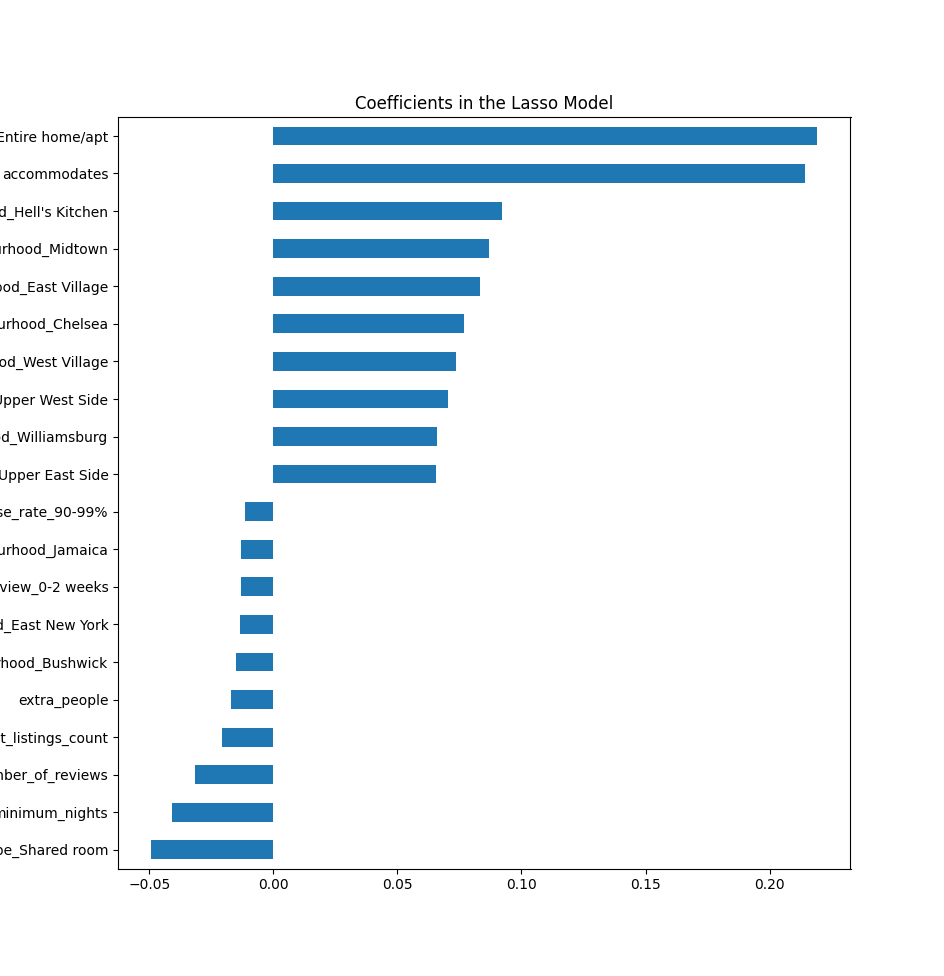
\includegraphics[width=\textwidth]{Figure_19.png}
    \label{fig:lasso-feature-importantance}
\end{figure}


It is not surprising that the two most important positive features are whether
the type of listing is the entire home and how many people the property
accommodates. These are the main things a customer would use to search for
properties in the first place.
Features related to the location are in the top 10.  Being in  Hell's
Kitchen, Midtown, East Village, Chelsea, West Village, Upper West Side,
Williamsburg, Upper East Side, SoHo, Lower East Side neighbourhood is associated
with an increase in the listing price.

\subsection{XGboost}

As shown by the Table ~\ref{tab:results}, XGboost consistently outperforms these
competing approaches in both mean squared error and R-squared.  With this model,
the features explain approximately 73\% of the target variable's variance and
have smaller MSE than the other regression model.

%Apart from its superior performance, another advantage of applying ensembles of
%decision tree methods like gradient boosting is that they can automatically
%provide estimates of feature importance from a trained predictive model.
%as shown in Figure ~\ref{fig:xgboost-feature-importantance}.
%\begin{figure}[h]\centering
    %\caption{XGboost Feature Importance}
    %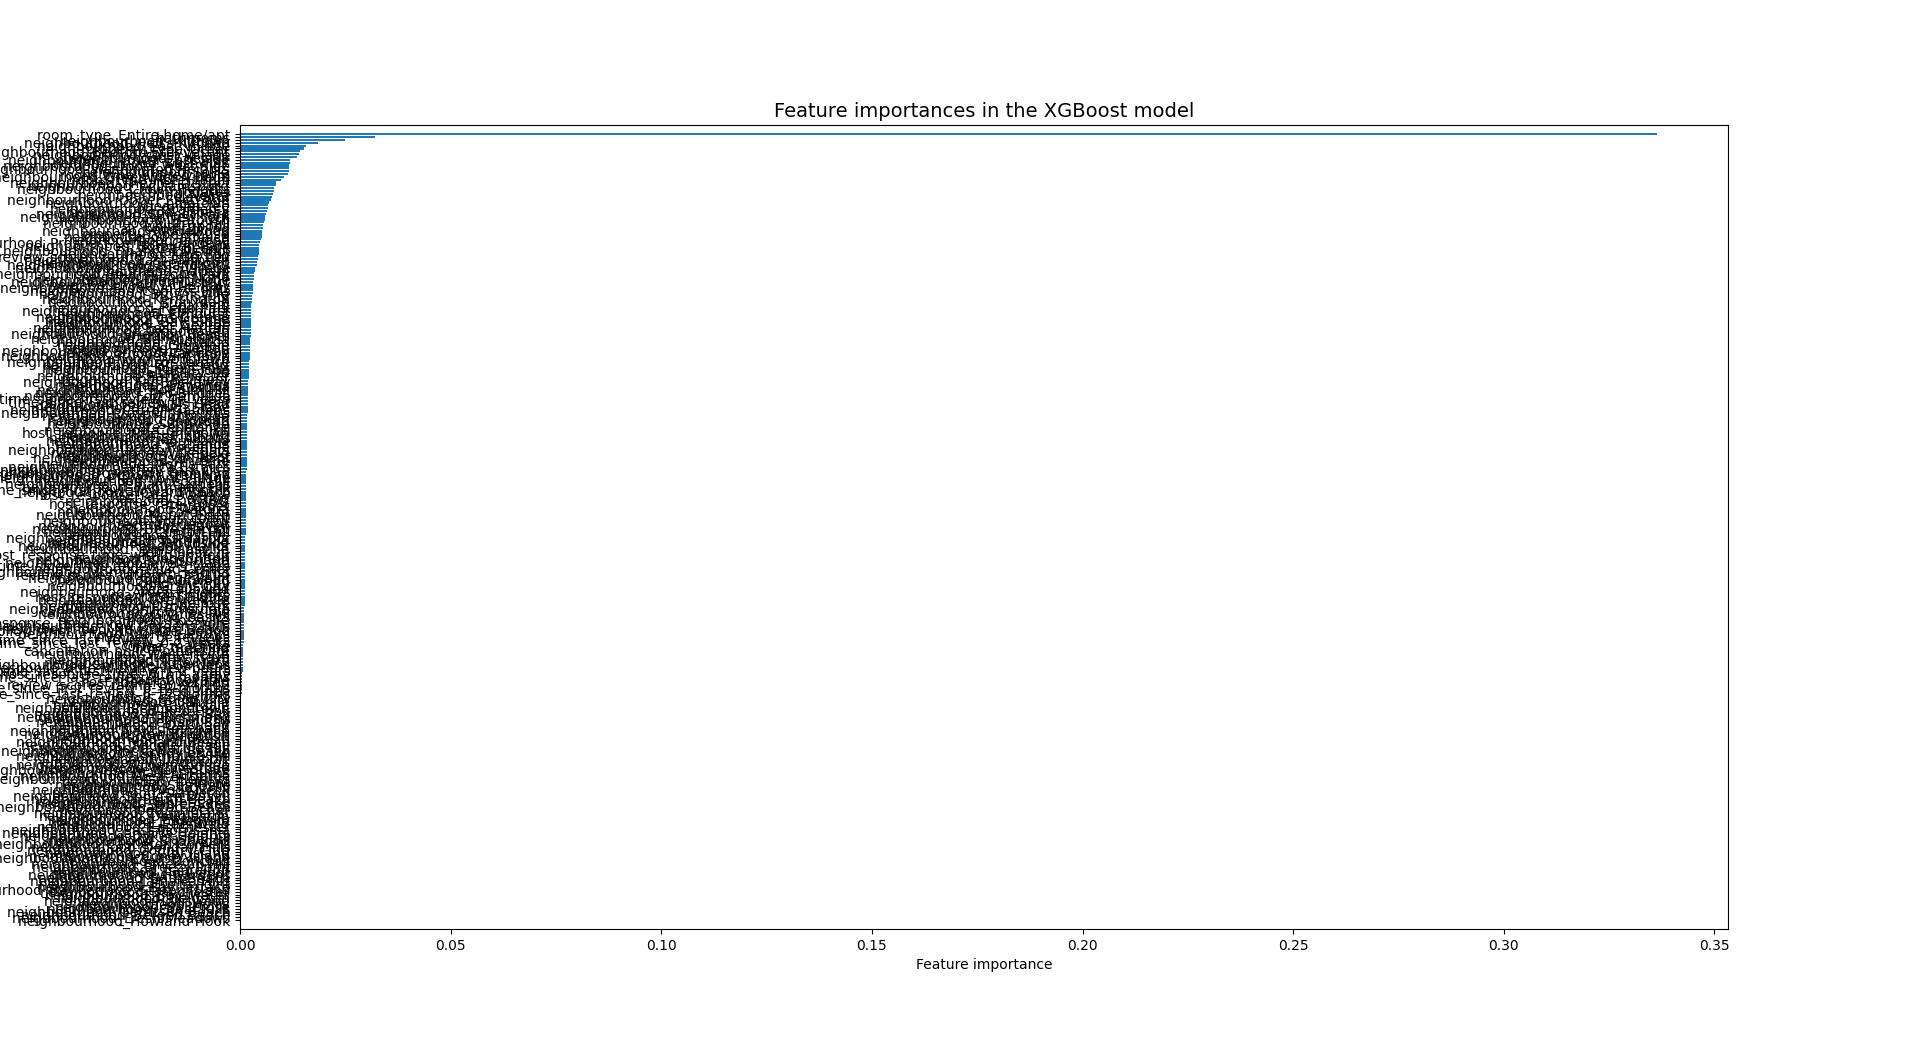
\includegraphics[width=\textwidth]{Figure_18.png}
    %\label{fig:xgboost-feature-importantance}
%\end{figure}

\begin{table}[H]
  \centering
  \caption{XGBoost Top 20 Feature Weights}
  \label{tab:xgb-weights}
  \begin{tabular}{lr}
    \toprule
    {} &    weight \\
    \midrule
    room\_type\_Entire home/apt        &  0.336396 \\
    bathrooms                        &  0.032001 \\
    neighbourhood\_Midtown            &  0.025008 \\
    neighbourhood\_Hell's Kitchen     &  0.018545 \\
    neighbourhood\_East Village       &  0.015763 \\
    property\_type\_Other              &  0.015168 \\
    neighbourhood\_Bedford-Stuyvesant &  0.014314 \\
    neighbourhood\_West Village       &  0.014031 \\
    neighbourhood\_Chelsea            &  0.013612 \\
    neighbourhood\_Lower East Side    &  0.011874 \\
    neighbourhood\_Bushwick           &  0.011854 \\
    neighbourhood\_Upper West Side    &  0.011682 \\
    neighbourhood\_Washington Heights &  0.011659 \\
    neighbourhood\_SoHo               &  0.011582 \\
    room\_type\_Shared room            &  0.011304 \\
    neighbourhood\_Greenwich Village  &  0.010347 \\
    room\_type\_Hotel room             &  0.009697 \\
    neighbourhood\_Theater District   &  0.008575 \\
    neighbourhood\_Williamsburg       &  0.008490 \\
    neighbourhood\_Crown Heights      &  0.007979 \\
  \bottomrule
  \end{tabular}
\end{table}

